
\documentclass[11pt]{article}

\usepackage{common}
\usepackage{amsfonts}
\usepackage{hyperref}
\title{HW5: Named Entity Recognition}
\author{Colton Gyulay \\ cgyulay@college.harvard.edu }
\begin{document}

\maketitle{}
\section{Introduction}

In the fifth problem set, our goal was to implement sequential language models in order to predict entity types across sentences. Formally, this task can be called named entity recognition (NER) as we are looking to classify chunks of text into five broad entity groups: non-entity, person, location, organization, and miscellaneous. Three primary types of models were built for this task: a simple hidden Markov model (HMM), a maximum-entropy Markov model (MEMM), and a structured perceptron (SP). All models are influenced by prior work on this task, as detailed by \citet{tjong2003introduction}, a broad report covering model performances and structure from the Conference on Computational Natural Language Learning (CoNLL).

The first class of models relied on assembling a context/class co-occurrence matrix to make entity predictions. This approach is limited in that it is more easily confounded by unseen contexts during validation and test. The MEMM, which is essentially a logistic regression model, and the SP utilized learned embeddings for vocabulary and previous classes to generalize better to unseen inputs. All models relied on the Viterbi algorithm (see \citet{DBLP:journals/corr/abs-cs-0504020}) to generate maximum-likelihood entity predictions across sequences. Though Viterbi was only used for HMM and MEMM testing, it was used directly in SP training.

\section{Problem \& Model Descriptions}

\subsection{Dataset}

The primary training dataset used was from CONLL, which is a collection of sentences tagged with word-level BIO chunk information. The dataset contained around 75,000 words across training and validation splits and had a vocabulary $\mcV$ of 15,700. The number of prediction classes $mcC$ was 9, which corresponded to one empty tag, two artificial start and end of sentence tags, four "I" tags relating to Person, Location, Organization, and Miscellaneous, and two further "B" tags for Location and Miscellaneous, which were used to indicate the start of a new tag contiguous to an existing tagging chunk.

\subsection{HMM}

The HMM structure relied on two primary matrices: a word/entity co-occurrence matrix $\boldE \in \reals^{|V| \times |C|}$ which models emission probabilities, and a previous entity/current entity co-occurrence matrix $\boldT \in \reals^{|C| \times |C|}$ which models transition probabilities. The probability of any entity label is then the product of the emission and transition probabilities given a certain context. This model is able to produce impressive results with only one pass over the training data, though it doesn't generalize as well when confronted with new vocabulary. This model, as well as the MEMM and SP models, utilized a Markovian assumption where entity predictions were only made given information of the current word and previous entity label.

\subsection{MEMM}

Moving on from the more naive HMM approach, we built a maximum-entropy Markov model which closely follows the structure of a logisitic regression model. The MEMM seeks to learn vector representations for words and classes in order to perform entity predictions. To generate a predicted distribution, the current word and the previous entity label were fed into parallel lookup tables, which essentially represent a linear transformation. The word lookup was handled by a learned weight matrix $\boldW^{w} \in \reals^{|V| \times |C|}$ while the class lookup was handled by a learned weight matrix $\boldW^{c} \in \reals^{|C| \times |C|}$. Representations were then added and converted to log probabilities $p \in \reals^{|C|}$ with the use of the $LogSoftMax$ function, which normalizes by dividing each entry by the sum of the log probability predictions. Given an input word $x$ and previous entity label $c$, the model can be formalized as follows:
\begin{center}
    $MEMM(x, c) = logsoftmax(\boldW^{w}x + \boldW^{c}c)$
\end{center}

Traditionally, \textit{LogSoftMax} is problematic as it requires summing over all output classes $\mcC$ for each example. Because of our relatively small $|\mcC|$, training was fast and we didn't need to employ tricks such as hierarchical SoftMax.

\subsection{Structured Perceptron}

The structured perceptron follows a very similar structure to the MEMM, though it differed primarily in training. Predictions were again generated by feeding current words and previous entity labels to weight matrices $W^{w}$ and $W^{c}$ respectively. Scores, however, were not normalized by $LogSoftMax$, but were instead used directly with the Viterbi algorithm to choose entity labels over an input sequence. During training, these entity labels were then compared to correct sequences, and a gradient was constructed by hand. The gradient penalized mismatches between the predicted and correct entity labels by increasing weights associated with correct entity labels and decreasing weights associated with incorrect labels. Matching predictions resulted in no gradients. The final structure can be seen formalized below:
\begin{center}
    $SP(x, c) = \boldW^{w}x + \boldW^{c}c$
\end{center}

\section{Model Structure \& Training}

A high level description of each model was given in the previous section, and here we will more formally present the topology and code used to build each of our models. The HMM primarily utilized word/entity and previous entity/current entity co-occurrence  matrices, for which the Torch code is as below. Counts were then normalized to log probabilities for prediction.
\begin{verbatim}
local transition = torch.zeros(nclasses, nclasses) -- p(y_{i}|y_{i-1})
local emission = torch.zeros(nwords, nclasses) -- p(x_{i}|y_{i})

for i = 1, train_x:size(1) do
  local x = chop(train_x[i])
  local y = chop(train_y[i])

  for j = 1, x:size(1) do
    local word = x[j]
    local class = y[j]
    emission[word][class] = emission[word][class] + 1

    if j < x:size(1) then
      transition[y[j+1]][class] = transition[y[j+1]][class] + 1
    end
  end
end
\end{verbatim}

The Torch implementation of the basic MEMM closely follows the mathematical formalization in the previous section. The model belows uses word and class embeddings, which are then combined and fed to a $LogSoftMax$ which converts class scores to log probabilities.
\begin{verbatim}
nn.Sequential {
  [input -> (1) -> (2) -> (3) -> output]
  (1): nn.ParallelTable {
    input
      |`-> (1): nn.Sequential {
      |      [input -> (1) -> (2) -> output]
      |      (1): nn.LookupTable
      |      (2): nn.Sum
      |    }
      |`-> (2): nn.Sequential {
      |      [input -> (1) -> (2) -> output]
      |      (1): nn.LookupTable
      |      (2): nn.Reshape(9)
      |    }
       ... -> output
  }
  (2): nn.CAddTable
  (3): nn.LogSoftMax
}
\end{verbatim}

The Torch implementation of the SP is given below. It closely mirros the MEMM structure, though does not utilize a $LogSoftMax$ layer for normalization.
\begin{verbatim}
nn.Sequential {
  [input -> (1) -> (2) -> output]
  (1): nn.ParallelTable {
    input
      |`-> (1): nn.Sequential {
      |      [input -> (1) -> (2) -> output]
      |      (1): nn.LookupTable
      |      (2): nn.Sum
      |    }
      |`-> (2): nn.Sequential {
      |      [input -> (1) -> (2) -> output]
      |      (1): nn.LookupTable
      |      (2): nn.Reshape(9)
      |    }
       ... -> output
  }
  (2): nn.CAddTable
}
\end{verbatim}

\subsection{Training}
The HMM required only a single epoch of training to model probabilities in the underlying data, while the MEMM and SP took a number of passes over the data to learn adequate functions. The MEMM was trained using mini-batch stochastic gradient descent and still trained relatively rapidly given the tractable size of $\mcC$.

Training of the structured perceptron was far more in-depth, and we employed a few tricks to ensure stability during learning. Instead of using small randomized lookup weights at initialization, weights were set to 0 and adjusted manually for each input sequence. For every training example, an optimal sequence was predicted using Viterbi, and then each incorrect prediction was adjusted as specified earlier. Without any modification, performance varied significantly from epoch to epoch, even with a heavily reduced learning rate. The relative weights learned were simply too chaotic to learn a well-fitting function for the data. To combat this, we devised a momentum system using a memory coefficient $m$, which struck a balance between using strict vanilla gradient descent ($m=0$) and no learning of new parameters ($m=1$). We found a coefficient of 0.8 to be optimal, which largely discarded new updates but learned enough to find a stable manifold.

\subsection{Evaluation}
Though model training was primarily observed through validation on accuracy and validation sets, this is not an adequate scoring function for entity chunk labeling. Instead, the F score, specifically the F1, was employed to monitor each model's precision and recall on held out data. F1 equally weights precision (the correctness of positive predictions) and recall (the correct percentage of positive predictions).

\section{Experiments}

In total, the HMM and SP models outperformed the MEMM, though surprisingly the HMM outperformed both more sophisticated approaches. The HMM and SP achieved similar F1 scores on the named entity chunking task, posting F1 results of \textbf{65.7} and \textbf{59.9} respectively. The MEMM lagged slightly behind, posting a best performance of only \textbf{45.1}. The SP, however, achieved very high training and validation accuracy, which indicates it was able to learn the patterns necessary for prediction fairly well, even if it failed to adequately generalize to the true entity recognition task.

\subsection{HMM}
In order to better handle unseen contexts, we utilized a Laplacian smoothing constant $\alpha$ which gave probability mass to these contexts. Tuning of this constant found an optimal score around $\alpha=0.2$ for emission and transition modeling. \textit{Figure 1} illustrates this curve. Our best HMM recorded a validation F1 score of \textbf{65.7}.

\begin{center}
    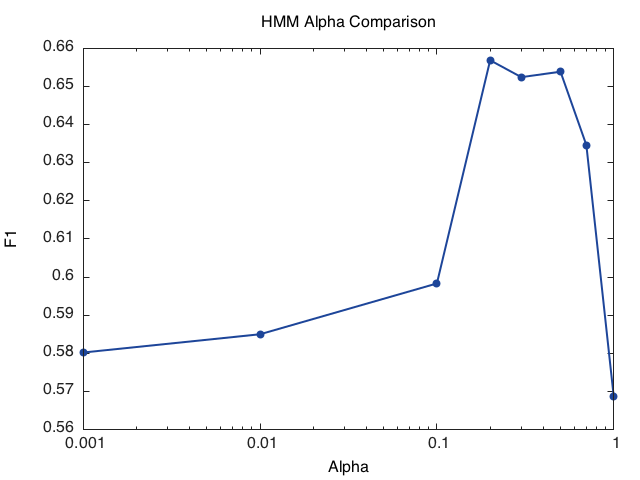
\includegraphics[width=12cm]{alphacomp.png}\\
    \textit{Figure 1: Comparing $\alpha$ values for HMMs.}
\end{center}

\subsection{MEMM}

With the MEMM we mainly experimented with the learning rate $\eta$ in order to maximize performance. Training for the MEMM, however, wasn't directly related to the entity labeling task as it sought to maximize accuracy over training data instead of the desired F1 score. Though the MEMM was able to achieve very high training and validation accuracy, it did not improve upon the HMM in F1 performance. Interestingly, we found a very high learning rate of $\eta=3$ to produce the best results on validation F1. \textit{Figure 2} demonstrates a comparison of different learning rates, while \textit{Figure 3} demonstrates training and validation performance. The MEMM did not overfit training data, though it did overfit the accuracy task and did not perform as well on F1 score as other models.

\begin{center}
    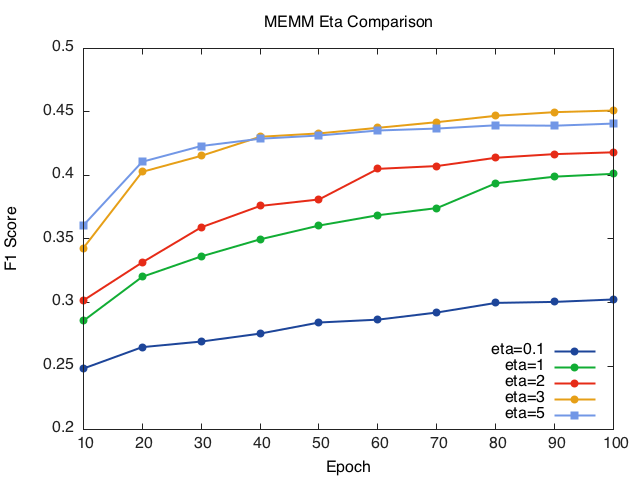
\includegraphics[width=12cm]{memmetacomp.png}\\
    \textit{Figure 2: Comparing MEMMs with different $d\eta$ values.}
\end{center}

\begin{center}
    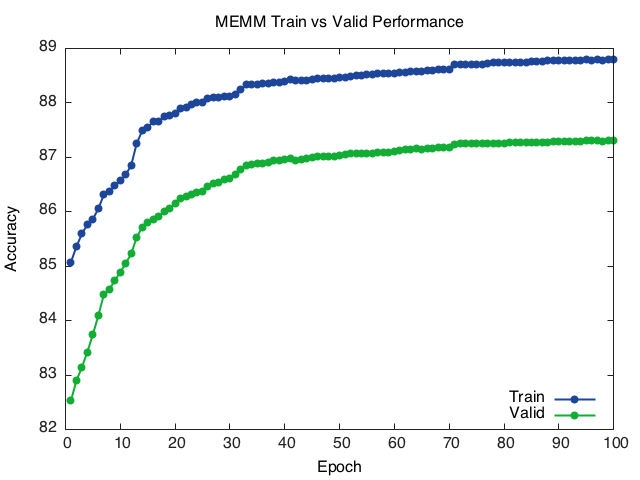
\includegraphics[width=12cm]{memmacc.png}\\
    \textit{Figure 3: MEMM training and validation accuracy.}
\end{center}

\subsection{SP}

During structured perceptron experimentation, we mainly examined the effects of cross-epoch weight preservation to induce better training stabilization. \textit{Figure 4} compares standard stochastic gradient descent, which jumps around during training, with momentum based learning, which is significantly more stable. Though a number of different values were tried for $\eta$, these did not make a huge difference in performance. This is likely due to the learned decision boundaries relying more on the weights relative to one another. When the model utilized a larger preference for maintaining older weights, it performed better. The maximum memory $m=1$, however, results in no learning by definition. \textit{Figure 4} compares SP performance across different values for $m$. Finally, the best results across all different models can be seen in \textit{Table 1}.

\begin{center}
    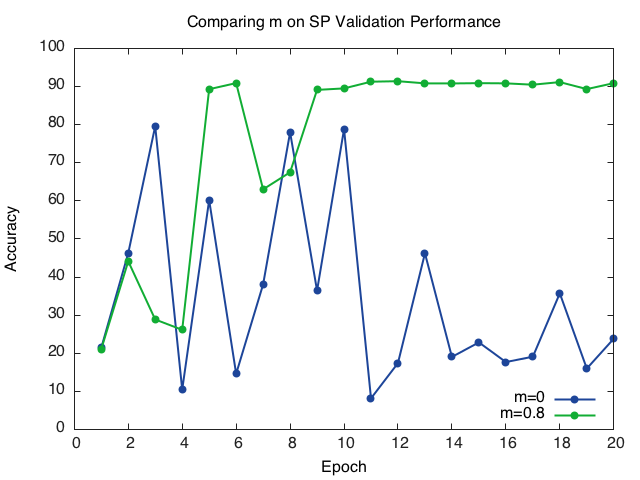
\includegraphics[width=12cm]{spcomp.png}\\
    \textit{Figure 4: Comparing SP models of different $m$ values.}
\end{center}

\begin{table}[h]
\centering
\begin{tabular*}{0.85\textwidth}{@{\extracolsep{\fill} }| c | c | c | c |}
\toprule
Model & CoNLL (Train Acc) & CoNLL (Valid Acc) & CoNLL (Valid F1)\\
\midrule
\textsc{HMM} & - & - & \textbf{65.7}\\
\textsc{MEMM} & 88.8 & 87.3 & 45.1\\
\textsc{SP} & 93.6 & 90.9 & 59.9\\
\bottomrule
\end{tabular*}
\caption{\label{tab:results} Training, validation, and F1 performance of model variants.}
\end{table}

\section{Conclusion}

In conclusion, we were able to achieve solid results across our different models, though the maximum-entropy Markov model lagged behind the hidden Markov model and structured perceptron. The simple count-based approach of the HMM achieved impressive performance with much simpler training required by either the MEMM or SP. Interestingly, the SP proved very unstable during training without using weights averaged from epoch to epoch. Though it might be expected, a lower learning rate did not combat this issue as well as weight averaging.

The high validation accuracy exhibited by the SP seems to indicate that it should have outperformed the other models on the named entity F1 score. This lack of translation to the primary task is likely due to its accuracy at predicting non-entities, which doesn't translate to F score. Though greedy search was solely employed while using the Viterbi algorithm, beam search would be an interesting alternative to explore for sequence selection during prediction, and might even allow better performance from all three models. All code can be found on GitHub here \url{https://github.com/cgyulay/cs287/tree/master/HW5}, while Kaggle submissions can be found under the team name "Kid CUDA".

\bibliographystyle{apalike}
\bibliography{writeup}

\end{document}
